\documentclass{beamer}

\mode<presentation> {

%\usetheme{default}
%\usetheme{AnnArbor}
%\usetheme{Antibes}
%\usetheme{Bergen}
%\usetheme{Berkeley}
%\usetheme{Berlin}
%\usetheme{Boadilla}
%\usetheme{CambridgeUS}
%\usetheme{Copenhagen}
%\usetheme{Darmstadt}
%\usetheme{Dresden}
%\usetheme{Frankfurt}
%\usetheme{Goettingen}
%\usetheme{Hannover}
%\usetheme{Ilmenau}
%\usetheme{JuanLesPins}
%\usetheme{Luebeck}
\usetheme{Madrid}
%\usetheme{Malmoe}
%\usetheme{Marburg}
%\usetheme{Montpellier}
%\usetheme{PaloAlto}
%\usetheme{Pittsburgh}
%\usetheme{Rochester}
%\usetheme{Singapore}
%\usetheme{Szeged}
%\usetheme{Warsaw}

% As well as themes, the Beamer class has a number of color themes
% for any slide theme. Uncomment each of these in turn to see how it
% changes the colors of your current slide theme.

%\usecolortheme{albatross}
%\usecolortheme{beaver}
%\usecolortheme{beetle}
%\usecolortheme{crane}
%\usecolortheme{dolphin}
%\usecolortheme{dove}
%\usecolortheme{fly}
%\usecolortheme{lily}
%\usecolortheme{orchid}
%\usecolortheme{rose}
%\usecolortheme{seagull}
%\usecolortheme{seahorse}
%\usecolortheme{whale}
%\usecolortheme{wolverine}

%\setbeamertemplate{footline} % To remove the footer line in all slides uncomment this line
%\setbeamertemplate{footline}[page number] % To replace the footer line in all slides with a simple slide count uncomment this line

%\setbeamertemplate{navigation symbols}{} % To remove the navigation symbols from the bottom of all slides uncomment this line
}

\usepackage{graphicx} % Allows including images
\usepackage{booktabs} % Allows the use of \toprule, \midrule and \bottomrule in tables
\usepackage[utf8]{inputenc}

%----------------------------------------------------------------------------------------
%	TITLE PAGE
%----------------------------------------------------------------------------------------

\title[Transchiffrement SSL/TLS]{Transchiffrement SSL/TLS} % The short title appears at the bottom of every slide, the full title is only on the title page

\author{Bourdon, Générat, Hamdani, Souchal, Nouafo} % Your name
\institute[M2 SSI] % Your institution as it will appear on the bottom of every slide, may be shorthand to save space
{
Université de Rouen \\ % Your institution for the title page
\medskip
\textit{M2 SSI} % Your email address
}
\date{\today} % Date, can be changed to a custom date

\begin{document}

\begin{frame}
\titlepage % Print the title page as the first slide
\end{frame}

\begin{frame}
\frametitle{Overview} % Table of contents slide, comment this block out to remove it
\tableofcontents % Throughout your presentation, if you choose to use \section{} and \subsection{} commands, these will automatically be printed on this slide as an overview of your presentation
\end{frame}

%----------------------------------------------------------------------------------------
%	PRESENTATION SLIDES
%----------------------------------------------------------------------------------------

%------------------------------------------------
\section{Introduction}
\begin{frame}
\frametitle{Introduction}
\begin{itemize}
\item Contexte du projet
\item Intérêt du chiffrement
\item Problème pour l'entreprise
\end{itemize}
\end{frame}


\begin{frame}
\frametitle{Présentation du projet}
Solution proposée à l'entreprise
\begin{itemize}
\item Attaque de type MITM\footnote[frame]{Man In The Middle}
\item Analyser le trafic en clair
\item Compatible avec les IDS\footnote[frame]{Intrusion Detection System}
\end{itemize}
\end{frame}

\begin{frame}
\frametitle{Présentation du projet}
\begin{itemize}
\item 
\end{itemize}
\end{frame}
\begin{frame}
\frametitle{Gestion de projet}
\framesubtitle{Livrables}
\textbf{Les livrables}
\begin{itemize}
\item blabla
\end{itemize}

\textbf{Mode de livraison :}
\begin{itemize}
\item Cycle de développement en V
\item Démonstrations régulières de l'avancement :
\begin{description}

\item[30 janvier] Proxy HTTP, recherche collision simple
\item[6 février] Connexion SSL/TLS
\end{description}

\item Livraisons :
\begin{description}
\item[13 février] Livraison provisoire
\item[20 février] Livraison définitive
\end{description}
\end{itemize}

\end{frame}



\begin{frame}
\frametitle{Gestion de projet}
\framesubtitle{Les livrables et l'équipe}
\textbf{L'équipe}
\begin{itemize}
\item 5 étudiants
\item 3 sur la partie transchiffrement \textit{(Compétences : Java, protocole TLS, gestion des certificats}
\item 2 sur les collisions
\textit{(Compétences : C, fonction de hachage, génération de certificat}
\end{itemize}
\end{frame}


\begin{frame}
\frametitle{Gestion de projet}
\framesubtitle{Gestion des risques}
\begin{itemize}
\item 
\end{itemize}
\end{frame}


\begin{frame}
\frametitle{Gestion de projet}
\framesubtitle{Planification}
\begin{itemize}
\item 
\end{itemize}
\end{frame}


\section{Proxy SSL/TLS} 

\frame{
  \frametitle{Analyse}
  Cibles visées
    \begin{itemize}
      \item Réseau interne.
      \item Navigateurs web:
        \begin{itemize}
          \item Chrome 44\%
          \item Firefox 19\%
        \end{itemize}
    \end{itemize}
   Protocole SSL/TLS
     \begin{itemize}
       \item Protocole de sécurisation des échanges
       \item Mode client/serveur
       \item Authentification, confidentialité, intégrité
       \item Fragmentation des données
       \item HMAC pour l'intégrité
     \end{itemize}
}

\frame{
  \frametitle{Analyse}
     Record TLS
       \begin{itemize}
         \item Envoi: message-fragmentation-compression-HMAC-chiffrement
         \item Réception: déchiffrement-décompression-rassemblement
       \end{itemize}
     Handshake
       \begin{itemize}
         \item Négocier une session TLS
         \item Eléments d'une session
           \begin{itemize}
             \item session identifier
             \item peer certificate
             \item compression method
             \item cipher spec
             \item master secret
             \item Is resumable
           \end{itemize}
       \end{itemize}
}

\frame{
  \frametitle{Analyse}
  Etapes du Handshake
  \begin{itemize}
    \item Client Hello
    \item Server Hello
    \item Server Certificate
    \item Client Key Exchange
    \item Change Cipher Spec
  \end{itemize}
  
}

\frame{
  \frametitle{Conception}
  UML des classes Java
  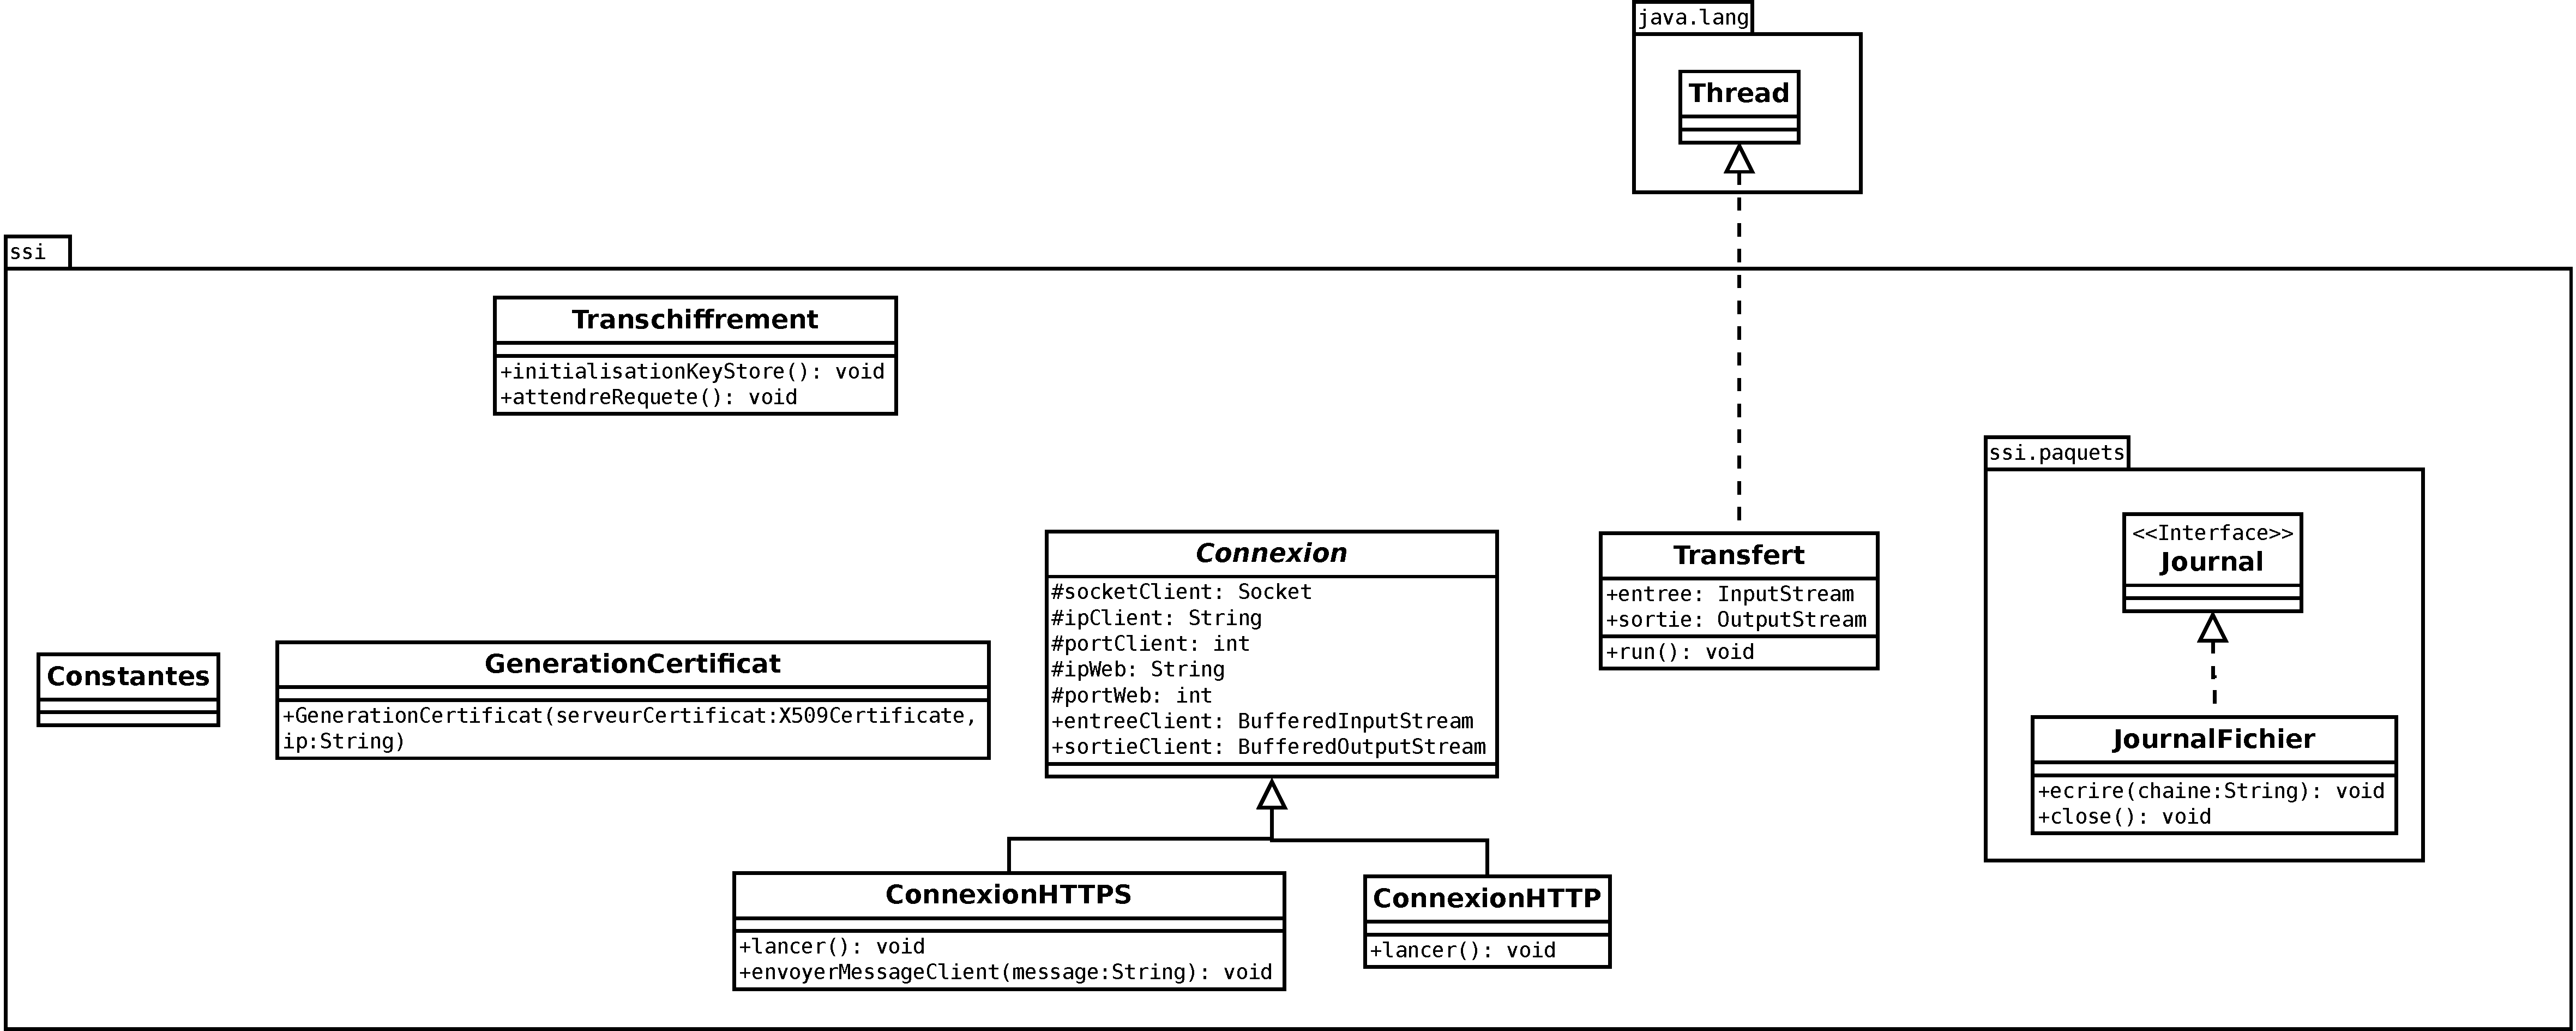
\includegraphics[width=\textwidth]{text/uml.pdf}
}

\frame{
  \frametitle{Accepter une autorité}
  Installer une autorité
  \begin{itemize}
    \item Utilisation d'un script
    \item Directement sur la machine utilisateur
    \item Dans le navigateur web du client
    \item Collision MD5
  \end{itemize}
  
  Collision MD5, vue d'ensemble
  \begin{itemize}
    \item Forge d'un faux certificat
    \item Signature identique
    \item Eviter l'installation d'une autorité
    \item Transparence maximale
  \end{itemize}
  
}

	\begin{frame}
		\frametitle{Threads}		
		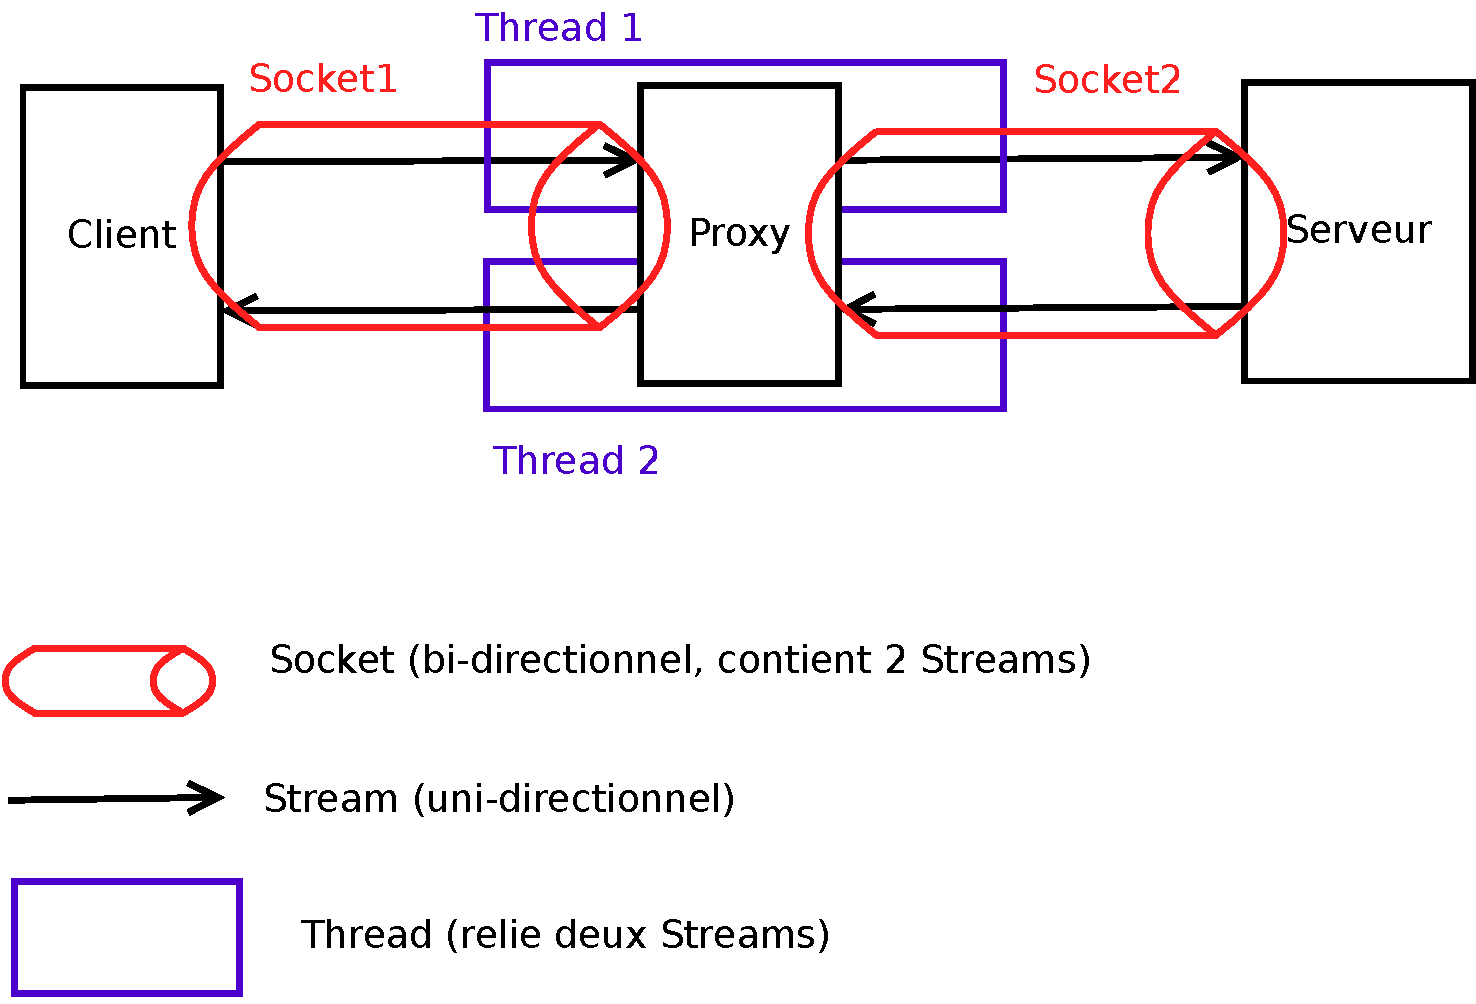
\includegraphics[width=\textwidth]{images/thread.pdf}
	\end{frame} 

	
	\begin{frame}
		\frametitle{Sockets}	
		\framesubtitle{Types de sockets dans Java}
		\begin{itemize}
			\item Socket
			\item SSLSocket
			\item ServerSocket
			\item SSLServerSocket
		\end{itemize}
	\end{frame} 
	
	\begin{frame}
		\frametitle{Sockets}	
		\framesubtitle{Utilisation en HTTP}
		\begin{itemize}
			\item Entre Client et Proxy \textit{Rôle serveur}
			\begin{itemize}
				\item Nécessité d'une ServerSocket en écoute.
				\item Création d'une Socket à la suite d'une connexion.
			\end{itemize}
			\item Entre Proxy et Serveur \textit{Rôle client}
			\begin{itemize}
				\item Récupération de l'ip et du port du serveur.
				\item Création d'une Socket pour se connecter au serveur.
			\end{itemize}
		\end{itemize}
	\end{frame}

	\begin{frame}
		\frametitle{Sockets}	
		\framesubtitle{Utilisation en HTTPS}
		\begin{itemize}
			\item Entre Client et Proxy \textit{Rôle serveur}
			\begin{itemize}
				\item Même déroulement que pour HTTP au début.
				\item Transformation de la Socket en SSLSocket en utilisant un Keystore pour trouver le certificat adéquat.
			\end{itemize}
			\item Entre Proxy et Serveur \textit{Rôle client}
			\begin{itemize}
				\item Même déroulement que pour HTTP au début.
				\item Création d'une SSLSocket pour se connecter au serveur et récupérer son certificat.
			\end{itemize}
		\end{itemize}
	\end{frame}

	\begin{frame}
		\frametitle{Keystore}
		\framesubtitle{Création}
		\begin{itemize}
			\item Sert à gérer les certificats pour les connexions sécurisées.
			\item Contient les autorités de certification reconnues par Java.
			\item Contient également notre autorité qui signera les faux certificats.
		\end{itemize}
	\end{frame} 
	
 		\begin{frame}
		\frametitle{Keystore}
		\framesubtitle{Utilisation}
		\begin{itemize}
			\item Génération d'un certificat semblable à celui du serveur.
			\item Création d'un fichier PKCS\#12 contenant ce certificat.
			\item Création d'un nouveau KeyStore à partir de ce PKCS\#12.
		\end{itemize}				
	\end{frame}
	
	\begin{frame}
		\frametitle{Journalisation}
		\begin{itemize}
			\item Récupération du trafic en clair dans un fichier.
			\item Précision sur l'heure et le sens de l'envoi.
		\end{itemize}				
	\end{frame} 
	
	

\section{Recherche de collisions sur des certificats hachés en MD5}
\begin{frame}
\frametitle{Fonction de hachage}


\begin{itemize}
\item A partir d'une donnée fournie en entrée, calcule un haché.\\
\item Résistance au calcul de pré-image.
\item Résistance au calcul de seconde pré-image.
\item Résistance au calcul de collision.\\
\end{itemize}
\end{frame}

\begin{frame}
\frametitle{Présentation MD5}

\begin{itemize}
\item Ronald Rivest en 1991.\\
\item Empreinte est de 128 bits.\\
\item Attaque par collision.
\end{itemize}
\end{frame}

\begin{frame}
\frametitle{schéma Merkle-Damgard}
\begin{figure}[h!]
\center
 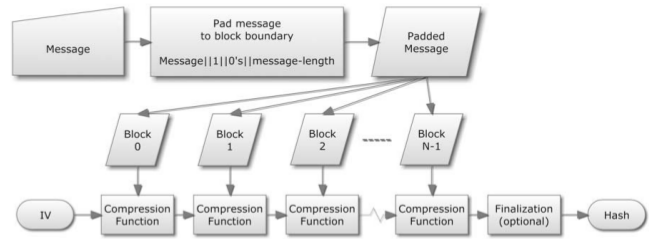
\includegraphics[width=11.5cm]{images/md.png}
 
  \caption{Principe de fonctionnement MD5}
\end{figure}
\end{frame}


\begin{frame}
\frametitle{Vulnérabilité MD5}

\begin{itemize}
\item Wang et Yu (2004).\\
\item Marc Stevens (2007).\\
\end{itemize}
\end{frame}
\begin{frame}
		\frametitle{Attaque de Wang}		
		\begin{block}{Type d'attaque}
		\begin{itemize}
		\item attaque par collision
		  \begin{itemize}
		  \item trouver M = ($M_0, M_1$) et M' = ($M'_0, M'_1$) tel que MD5(M) = MD5(M')
		  \end{itemize}
		\item Utiliser une m\'ethode dite diff\'erentielle
		 \begin{itemize}
		 \item analyser les diff\'erences fix\'ee entre deux messages 
		 \end{itemize}
		\end{itemize}
		\end{block}
		
		\begin{block}{Caract\'erisation}
		\begin{itemize}
		\item (a, b, c, d) = MD5($a_0, b_0, c_0, d_0, M_0$)
		\item (a', b', c', d') = MD5($a_0, b_0, c_0, d_0, M'_0$)
		\item on a MD5($a, b, c, d, M_1$) = MD5($a', b', c', d', M'_1$).
\end{itemize}
		\end{block}
	\end{frame}

	\begin{frame}
		\frametitle{D\'eroulement de l'attaque}
		\begin{block}{Condition pour mener l'attaque}
		  \begin{enumerate}
		  \item Diff\'erence entre les premiers blocs de 512 bits 
		    \begin{itemize}
		    \item $\Delta$$M_{0}$ = $M'_{0}$ - $M_{0}$ = (0, 0, 0, 0, $2^{31}$ , 0, 0, 0, 0, 0, 0, $2^{15}$, 0, 0, $2^{31}$, 0)
		    \end{itemize}
%		  \item Diff\'erence entre les seconds blocs de 512 bits 
		    \begin{itemize}
		    \item $\Delta$$M_{0}$ = $M'_{0}$ - $M_{0}$ = (0, 0, 0, 0, $2^{31}$, 0, 0, 0, 0, 0, 0, -$2^{15}$, 0, 0, $2^{31}$, 0)
		    \end{itemize}
		  \item Diff\'erence entre les signatures des deux premiers blocs
		   \begin{itemize}
		   \item $\Delta$$IV_{1}$ = $IV'_{1}$ - $IV_{1}$ = ($2^{31}$, $2^{31}$ + $2^{31}$, $2^{15}$ + $2^{31}$, $2^{15}$ + $2^{31}$)
		   \end{itemize}

		  \end{enumerate}
		\end{block}
	
		\begin{block}{R\'esum\'e}
		 \begin{itemize}
		 \item Ne permet pas le calcul de pr\'e-image.
		 \item M et M' sont deux messages de 1024 bits chacun.
		 \item M et M' sont obtenus apr\`es deux passages dans la fonction MD5Compress.
		 \item Complexité de recherche
		 \begin{itemize}
		 \item premier bloc: $2^{33}$
		 \item second bloc: $2^{29}$
		 \end{itemize}
		\end{itemize}
		\end{block}
	\end{frame} 




	\begin{frame}
		\frametitle{Attaque de Marc Stevens}
		\begin{block}{}
		  \begin{itemize}
		  \item S'appuie sur les recherches de Wang.
		  \item Permet le calcul de pr\'efixe.
		  \item Construction progressive des blocs de collisions.
		  \end{itemize}
		\end{block}
	
		\begin{block}{Caract\'erisation}
		  \begin{itemize}
		  \item Trouver M = P . S et  M' = P' . S' tel que MD5(M) = MD5(M').
		  \item (P, P') pr\'efixes de (M, M') dont les valeurs sont fixes.
		  \item (S, S') suffixes de (M, M')
		  \end{itemize}
		\end{block}
	\end{frame}

	
	\begin{frame}
		\frametitle{Attaque de Marc Stevens}
		\begin{block}{D\'ecomposition des suffixes S et S'}
		S et S' ont la m\^eme structure qui suit:
		  \begin{itemize}
		  \item $S_r$: padding choisit tel que P . $S_r$ . $S_b$ . $S_c$ multiple de 512.
		  \item $S_b$: bits d'anniversaires.
		  \item $S_c$: bits de quasi collisions.
		  \end{itemize}
		\end{block}
		
		\begin{block}{Condition pour mener l'attaque}
		  \begin{itemize}
		  \item Utilise la m\'ethode diff\'erentielle et des bits de conditions.
		    \begin{itemize}
		    \item Permet de calculer un chemin diff\'erentiel \`a partir de $\Delta$IHV et $\Delta$B.
		    \item Le chemin est d\'efini \`a l'aide de bits de conditions.
		    \end{itemize}
		  \end{itemize}
		  
		  La complexité de cette m\'ethode est de $2^{16}$ appels \`a la fonction de compression MD5.
		\end{block}
	\end{frame}
	
			
			
			
			
	\begin{frame}
		\frametitle{Application aux certificats}
		\begin{block}{Points essentiels}
		  \begin{itemize}
		  \item D\'etermination du pr\'efixe.
		  \item O\`u op\'erer la recherche des blocs de collisions.
		  \item Propagation des blocs de collisions.
		  \end{itemize}
		\end{block}
		
		\begin{block}{Principe}
		  \begin{itemize}
		  \item G\'en\'erer deux certificats \`a faire signer par l'autorit\'e: un vrai et un faux
		    \begin{itemize}
		    \item D\'eterminer le d\'ebut des modules RSA.
		    \item Modification du module RSA du faux pour en contr\^oler la cl\'e priv\'ee.
		    \end{itemize}
		  \end{itemize}
		\end{block}
		
	\frame{
	\frametitle{Exemple de certificats}
	
	}
	\end{frame}



\section{Démonstration}
\begin{frame}
\frametitle{Démonstration}
Notre mode opératoire
\begin{itemize}
%\item Installation du certificat chez un client avec un script
\item Navigation HTTP
\item Navigation HTTPS : observation des trames chiffrées et du flux déchiffré
\item Récupération du mot de passe
\end{itemize}
\end{frame}

\section{Conclusion}
\begin{frame}
\frametitle{Conclusion}
\begin{itemize}
\item Étude d'un protocole de communication sécurisé
\item Implémentation du protocole
\item Concepts cryptographiques associés
\end{itemize}
\end{frame}



\begin{frame}
\frametitle{Blocks of Highlighted Text}
\begin{block}{Block 1}
Lorem ipsum dolor sit amet, consectetur adipiscing elit. Integer lectus nisl, ultricies in feugiat rutrum, porttitor sit amet augue. Aliquam ut tortor mauris. Sed volutpat ante purus, quis accumsan dolor.
\end{block}

\begin{block}{Block 2}
Pellentesque sed tellus purus. Class aptent taciti sociosqu ad litora torquent per conubia nostra, per inceptos himenaeos. Vestibulum quis magna at risus dictum tempor eu vitae velit.
\end{block}

\end{frame}

%------------------------------------------------

\begin{frame}
\frametitle{Multiple Columns}
\begin{columns}[c] % The "c" option specifies centered vertical alignment while the "t" option is used for top vertical alignment

\column{.45\textwidth} % Left column and width
\textbf{Heading}
\begin{enumerate}
\item Statement
\item Explanation
\item Example
\end{enumerate}

\column{.5\textwidth} % Right column and width
Lorem ipsum dolor sit amet, consectetur adipiscing elit. Integer lectus nisl, ultricies in feugiat rutrum, porttitor sit amet augue. Aliquam ut tortor mauris. Sed volutpat ante purus, quis accumsan dolor.

\end{columns}
\end{frame}

\begin{frame}
\frametitle{Table}
\begin{table}
\begin{tabular}{l l l}
\toprule
\textbf{Treatments} & \textbf{Response 1} & \textbf{Response 2}\\
\midrule
Treatment 1 & 0.0003262 & 0.562 \\
Treatment 2 & 0.0015681 & 0.910 \\
Treatment 3 & 0.0009271 & 0.296 \\
\bottomrule
\end{tabular}
\caption{Table caption}
\end{table}
\end{frame}

\begin{frame}[fragile] % Need to use the fragile option when verbatim is used in the slide
\frametitle{Verbatim}
\begin{example}[Theorem Slide Code]
\begin{verbatim}
\begin{frame}
\frametitle{Theorem}
\begin{theorem}[Mass--energy equivalence]
$E = mc^2$
\end{theorem}
\end{frame}\end{verbatim}
\end{example}
\end{frame}



%------------------------------------------------

\begin{frame}
\Huge{\centerline{Merci de votre attention}}
\end{frame}

%----------------------------------------------------------------------------------------

\end{document} 